\section{Marco Teórico}

\subsection{Microcontrolador ATmega328P}



\subsection{Registros de propósito general}

\subsection{Entradas y Salidas Digitales}
\begin{itemize}
    \item Concepto de GPIO.
    \item Uso de pulsadores como entradas digitales (debouncing si es necesario).
    \item Uso de LEDs como indicadores de estado.
\end{itemize}


\subsection{Stack Pointer}
El stack pointer es una herramienta utilizada dentro de la programación del microcontrolador. El stack pointer es un no es nada más que un puntero interno del microcontrolador (similar a X, Y o Z) el cual tiene una serie de operaciones asignadas, y un comportamiento específico. El stack pointer se inicializa al final de la memoria RAM, alejado de todo para intentar no molestar al resto. Allí el stack pointer se % ... 

Instrucciones como call, rcall, o las interrupciones dependen de la inicialización previa del Stack Pointer, para poder funcionar de manera adecuada, ya que el Stack Pointer es el que se encarga de guardar las direcciones de memoria a las cuales estas instrucciones deben retornar luego de terminar la ejecución, de no estar inicializado el Stack Pointer, el programa no sabría a donde volver luego de una interrupción, muy probablemente yendo a una dirección del programa aleatoria y rompiendo el flujo del codigo.

\subsection{Delay activo}
Un delay activo es una pieza de código que toma en cuenta el la velocidad de ejecución del microcontrolador, para ejecutar un número de instrucciones (inútiles) concreto, representando un pasaje de tiempo específico, para luego retornar al flujo del programa. Son fáciles de usar, pero no es recomendable abusard de ellas debido a ineficiencias energéticas, y que el programa se mantiene ocupado la mayor parte del tiempo en el temporizador, en lugar de poder dedicarse a hacer otras tareas.

\subsection{Timers}
El atmega328p tiene 3 timers diferentes: Timer 0, Timer 1, y Timer 2.

Timer 0 y 2 son de 8 bits
Timer 1 es de 16 bits (puede contar más)

La ecuacion para calcular el tiempo del timer es la siguiente.

\begin{equation}
    \frac{(2^{k} - C_{\text{inicio}})\cdot \text{Prescaler}}{f_{\text{contador}}} = t_{\text{deseado}}
\end{equation}

Esta ecuación determina el tiempo que le tomaría al contador hacer un desbordamiento (overflow) en base a la frecuencia a la cantidad de bits del contador (k), la frecuencia de trabajo del microcontrolador, el tiempo o conteo con el que se inicie el contador, y el prescaler con el que esté configurado. 

\subsection{Interrupciones externas}

   \begin{figure}[H]
    \centering
    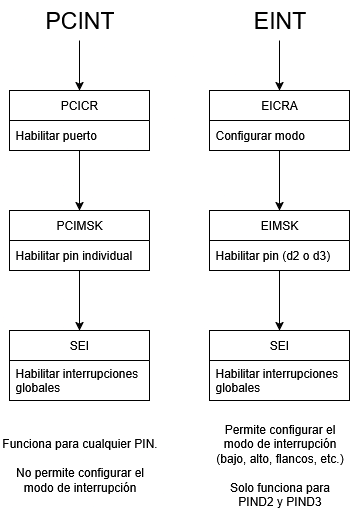
\includegraphics[width=0.7\linewidth]{./Anexos/Marco Teorico/External Interrupts/Interrupt diagram.png}
    \caption{Flujo de configuración de interrupciones exeternas. Fuente: Elaboración própia.}
    \label{fig:InterruptDiagram}
    \end{figure}


    \subsubsection{EINT}


    \subsubsection{PCINT}

\subsection{SRAM}

% Anexo: Como reservar sram
%       Como escribir sram
%       Como leer sram

Usando dseg se puede reservar espacio en memoria la SRAM para utilizarlo luego. Posteriormete con ``variable'' podremos leer o escribir el valor guardado con ``lds'' o ``sts'' respectivamente. O incluse se podría utilizar un puntero (X, Y, Z) para acceder a un lugar en memoria de manera iterativa donde quisieramos guardar múltiples valores subsecuentes (como un arreglo). 

Nota: Existen 2kb de memoria RAM, el stack pointer vive dentro de la RAM así que uno debe ser precabido con el uso excesivo de este recurso.

\subsection{FLASH}

Utilizando .cseg y una dirección segura como 0x300 para guardar datos, se puede utilizar la misma memoria FLASH para guardar datos constantes como LUTs, fotogramas, cadenas de texto, etc. Estos datos no pueden ser modificados, pero existen 32kb de espacio en memoria FLASH para guardar información, por lo que es menos limitante que la SRAM (2kb).

Para acceder a datos guardados en program memoria del programa (FLASH) se puede hacer haciendo uso del puntero Z y la instrucción ``lpm'':

% Anexo como guardar y leer de Flash

Se carga la dirección a Z cargando las partes bajas y altas de la dirección a ZL y ZH respectivamente. En los AVR  ``clásicos'' (como el ATmega328P), las etiquetas en memoria de programa (.cseg) están en direcciones de palabra (cada instrucción ocupa 16 bits), pero la instrucción LPM usa una dirección en bytes en el registro Z. Por eso se hace $<$$<$ 1 (multiplicar por 2): convierte la dirección en palabras de la etiqueta a dirección en bytes para LPM. Y ``Z+'' indica que luego de realizar lpm, se incremente en 1 el puntero ``Z''

\subsection{Bit masks}
Son numeros binarios pero lo que nos importa es la posición de los unos y ceros en lugar del valor mismo que representan. Un valor binario puede representar un número o una máscara, solo depende de como lo mires.  

``ldi r16, 0b00001010 out PORTB, r16'' carga una máscara de bits al puerto B para encender los pines 1 y 3, y apagar el resto, pero también se puede ver como que se está cargado el número 10 al puerto B (``ldi r16, 10 out PORTB, r16'')

Las máscaras son útiles cuando se busca afectar solo uno o varios de los bits de un registro. Lo que se hace primero es leer el registro, luego se realizar una operación lógica con la máscara que representa los bits que se quieren afectar, y por último se carga la máscara modificada al registro. Este tipo de operaciones se vuelve muy común cuando se trabajan con matrices LED, donde es muy común tener que mezclar puertos entre filas y columnas. Véase anexo % SET_BIT CLEAR_BIT


\subsection{LUT}
Para trabajar de manera ordenada en el desorden. Convierte al dolor de cabeza que son los puertos, en simples operaciones de lectura de FLASH, y modificación de punteros. Véase anexo %LUT



\begin{figure}[H]
  \centering
  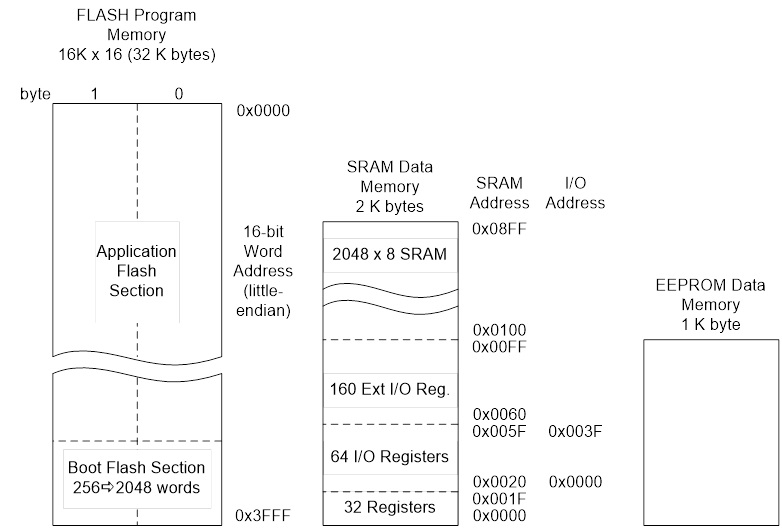
\includegraphics[width=\linewidth]{./Anexos/Memory Map.jpg}
  \caption{Mapa de memoria y espacios de direcciones en AVR de 8 bits. Fuente: \cite{arxterra_avr_addressing_modes}.}
  \label{fig:avr-memory-map}
\end{figure}

\subsection{USART asíncrono}

\subsection{Ring Buffer}

\subsection{USART asíncrono con Ring Buffer}

\subsection{Automatización y Máquinas de Estado}

\subsection{Kit FischerTechnik}

\begin{itemize}
    \item Principios básicos de una cinta transportadora en automatización.
    \item Funcionamiento de un actuador lineal/solenoide como punzón.
    \item Diferentes modos de operación según carga (ligera, media, pesada).
\end{itemize}


\subsection{Conversión Digital-Analógica (DAC R-2R)}
\begin{itemize}
    \item Concepto de DAC y su importancia.\vspace{0.5em}
    
    Un DAC (Digital to Analog Converter) es un dispositivo o técnica que permite transformar valores digitales (códigos binarios) en señales analógicas (tensiones o corrientes continuas y variables en el tiempo). Su importancia radica en que la mayoría de los sistemas electrónicos trabajan de manera digital, pero el mundo físico es analógico: audio, imágenes, señales de control de motores, etc.
    
    En pocas palabras, el DAC es el ``puente'' entre lo digital y lo analógico.\vspace{1em}

    \item Arreglo de resistencias R-2R.\vspace{0.5em}

    El arreglo R-2R es una red de resistencias que se usa mucho para construir DACs simples y económicos. Se compone unicamente de dos valores de resistencias: una de valor R y otra de valor 2R, que se repiten en forma de escalera.
    
    Cada bit de nel número digital controla un interruptor (o transistor) que conecta la red a una referencia de tensión (Vref) o a tierra. Gracias a la proporción entre Ry 2R, la red genera tenciones que corresponden al valor binario aplicado.
    
    La ventaja del arreglo R-2R es que es fácil de implementar, no requiere de resistencias con muchos valores distintos, y mantienen una buena presición.\vspace{1em}
    
    \item Uso de una Look-Up Table (LUT) para generar señales analógicas periódicas.\vspace{0.5em}
    
    Una Look-up Table (LUT) es básicamente una tabla de valores precargada en la memoria que representa una señal digitalizada (por ejemplo, una onda seno). En lugar de calcular cada valor de la función en tiempo real, el monitor solo ``lee'' la tabla en orden y envía los valores a un puerto o a un DAC.
    
    Cuando esos valores se aplican de manera periódica y con la velocidad adecuada, en la salida se reconstruye una señal analógica periodica.
    
    El uso de una LUT simplifica mucho la generación de señales, por que evita cálculos complejos y garantiza que la forma de onda siempre tenga la misma calidad.\vspace{1em}
\end{itemize}


\subsection{Matrices de LEDs}
Modelo
Anexo Pinout
Como prender un LED
Resistencias a utilizar



\subsection{Plotter y Control de Movimiento}
\begin{itemize}
    \item Concepto de plotter y su uso en ingeniería.
    \item Control de motores paso a paso o conmutados mediante relés/MOSFETs.
    \item Señales de control enviadas desde el microcontrolador a un PLC.
\end{itemize}
